\chapter{基于弱监督注意力的多人姿态估计方法}
\label{cha:method}

\section{概述}
\label{sec:methodoverview}
%   This part intends to state the overall idea
本方法使用基于残差网络\footnote{残差网络,简称ResNet, 全称Residual Network}与特征金字塔网络\footnote{特征金字塔网络,简称FPN, 全程Feature Pyramid Network}结构的网络框架作为特征提取的骨架,为模型提供各个尺度的特征图。在特征提取部分之后,网络可以分为目标检测与姿态估计和融合回归两个步骤。在目标检测与姿态估计过程中,网络预测出目标的边界框,粗略的关键点预测和实例分割结果。而在融合回归部分,网络会接受从目标检测与姿态估计阶段产生的结果并将它们一同以一定的方式互相交汇并一起回归。而且,在融合回归的过程中,网络采取了多阶段的堆叠和中继监督的策略来共同精炼关键点与实例分割的结果。这种结构是受到CPM\cite{wei2016convolutional}的启发而设计的。同时,为了有效地融合实例分割与姿态估计的结果,网络使用了注意力机制,使其根据实例分割的生成注意力关注网络对应的区域,从而达到方法最初设计的目的,也就是解决多人检测下姿态遮挡的问题。同时,考虑到姿态估计的信息对实例分割也有促进作用,本文设计了双流的网络结构让模型在每个阶段都能同时预测分割结果和姿态估计结果,并送入下一阶段继续优化。网络的整体结果如图\ref{fig:Overall}

%	ROI Extraction
%	key-point & Mask Prdiction
%		Stage One's Prediction
网络通过特征提取器$E$得到图像$I$来自网络各个尺度的特征$F=\{f_1, f_2, ..., f_5\}$。这些特征被兴趣区域对齐层\footnote{兴趣区域对齐层,简称RoI Align Layer, 全称Region of Interest Align Layer}通过双线性插值的方法调整到了同样的尺寸。每个图像中只有来自特定尺度$k$的特征图$f_k$被选中并被输入至接下来的目标检测与姿态估计部分。这个被选中的特征被分别送入了目标检测分支$D$与姿态估计分支$P$,分别得到了实例分割结果$S_1=\{s_1^1, s_1^2, ..., s_1^n\}$与姿态估计结果$K_1=\{k_1^1, k_2^1, ..., k_1^n\}$。这些中间结果会被输入到融合优化阶段进行多阶段的回归。

\begin{figure*}[htbp]	
	\centering
	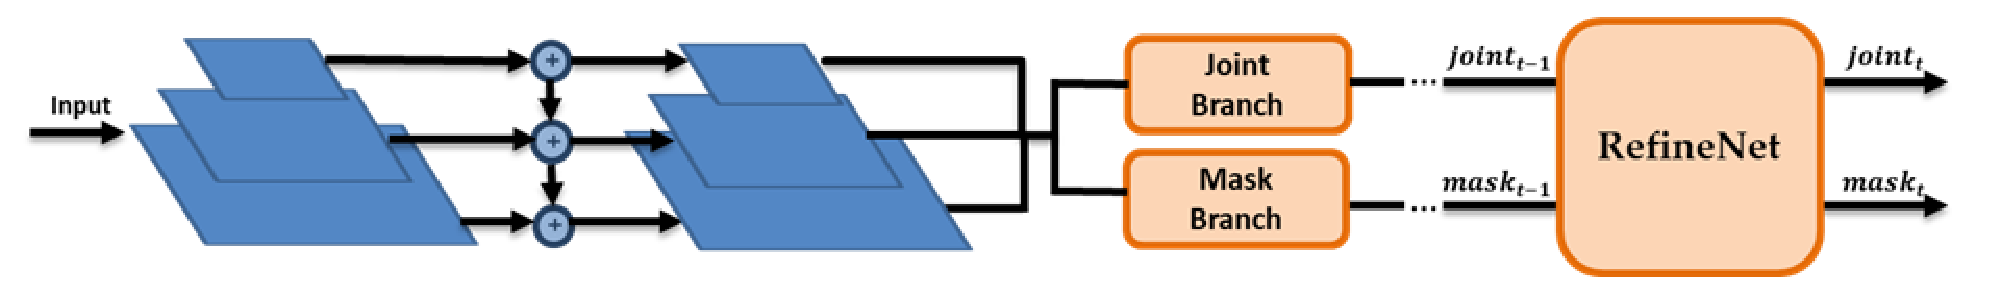
\includegraphics[scale=0.4]{network.eps}
	\caption{网络整体结构}
	\label{fig:Overall}
\end{figure*}

%		Stage 2+'s Prediction
如图\ref{fig:RefineNet}所示,在融合优化阶段的第$t(t>2)$阶段,单个优化模块接收来自特征提取器$E$的特征$f_k$、在阶段$t-1$中得到的姿态估计结果$K_{t-1}$与实例分割结果$S_{t-1}$。整个网络有主要设计亮点可以归纳为三点。第一是本文引入了注意力机制让网络关注具体的区域,本文设计了注意力转换模块来让生成一个合适的注意力与特征图融合,最后得到关键点预测结果$K_t$。第二,网络还会根据姿态估计的中间结果,也就是一些更偏向于得到关键点预测的特征,生成实例分割的结果。这让网络会根据来自姿态估计的信息修正实例分割的结果。最后,由注意力转换模块生成的注意力还会与从姿态估计那一支生成的中间结果融合,最终生成的实例分割的优化结果$S_t$。因此,整个优化模块$R$可以被抽象为形如公式\eqref{def:refinenet}的函数。


\begin{equation}
\label{def:refinenet}
M_t, K_t = R(M_{t-1}, K_{t-1})
\end{equation}

%   This part is to describe why we use a hybrid multi-stage arch
%	1. mask and key-point detection is associated
%	2. In crowd, the heatmap is not robust to predict
本方法使用了多阶段、利用弱监督约束的注意力的结构,同时优化实例分割与姿态估计的结果。首先多阶段与中继监督这两个设计可以让网络获得更大的感受野,让网络能够充分学习关键点之间的关系\cite{wei2016convolutional}。其次,由于实例分割和姿态估计是联系紧密的两个任务, 正如本文\ref{sec:generalmotivation}中提到的,实例分割与姿态估计能够相互优化,并且有相当大的相关性。所以这样设计的结构主要是希望能够同时优化姿态估计与实例分割结果。通过引入注意力以及弱监督这种较宽松约束下的可学习参数,网络能够更加适应数据中的不同表现。这让网络在一些实例分割无法正确引导关键点检测的情况下, 仍然能够生成较为正确的注意力引导关键点的检测与人体骨架的重建。

\begin{figure*}[htbp]	
	\centering
	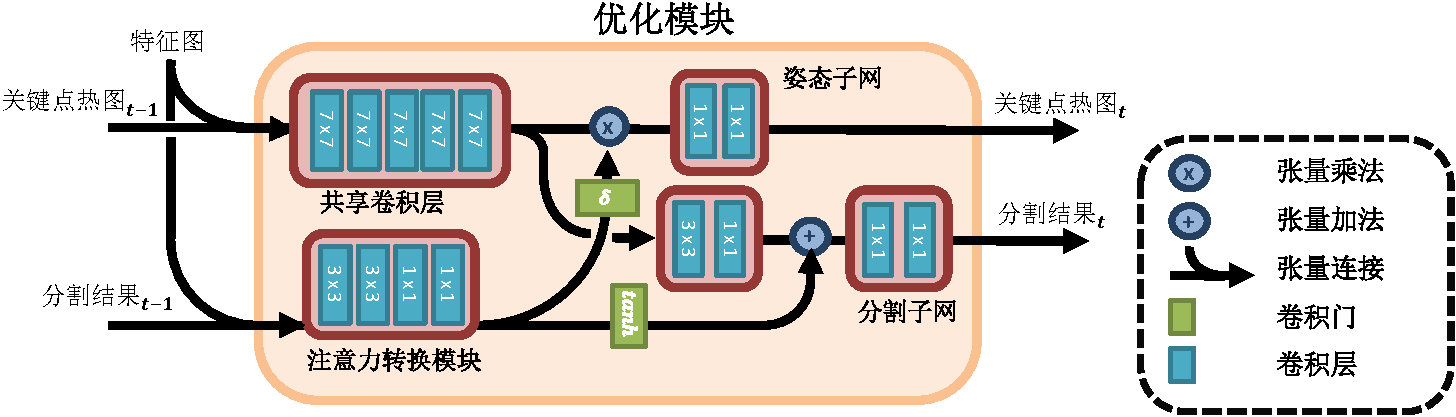
\includegraphics[scale=0.65]{RefineNet.pdf}
	\caption{融合优化模块具体设计}
	\label{fig:RefineNet}
\end{figure*}

\section{实例分割与姿态估计}
\label{sec:detectionstage}
%	Structure description
%	1. Hybrid arch of maskrcnn & cpm
本文在特征提取部分使用了101层的残差网络与特征金字塔网络来生成不同尺度的特征图供检测部分使用。正如Mask R-CNN\cite{He2017Mask}中使用的结构,本文也设计了并行的区域建议网络,在经过回归分支后从不同尺度的特征图上得到来自不同尺度的边界框。这些尺度不同的边界框会根据其来源送入专为特征金字塔网络设计的兴趣区域对齐层,根据公式选定对应的层数来裁剪并对齐特征图\cite{Lin2016Feature}。这样裁剪下来的特征图具有相对平衡的感受野:小尺寸物体有较小的感受野大小,同时大尺寸物体会获得更大的感受野大小。

检测部分是由两个并行的分支组成的。实例分割与姿态估计分支分别使用裁剪好的特征得到粗略的实例分割结果与姿态估计结果。分割分支的网络结构使用了四层卷积核大小为3像素的卷积层,和一层步长为2,卷积核大小为2的空洞卷积层。同样的,姿态估计分支使用了五层卷积核大小为3的卷积层,最终的输出被两层1x1卷积调整至关键点外加背景个通道,以得到每个关键点的热力图。

%   Training strategy description
%	Section 1
在检测部分的监督过程中,由于网络被设计为两个能够分别完成不同任务的并行分支,所以该部分的损失函数设计就表现为两个损失函数加和的形式。首先损失函数需要对目标位置检测进行监督,所以本文借鉴了区域卷积神经网络\cite{Girshick_2014_CVPR}中损失函数设计思路,使用交叉熵来计算预测标签与真实标签之间的距离。同样的,如Mask R-CNN\cite{He2017Mask}中的损失函数设计,交叉熵也被用来监督实例分割。

在检测部分中,由于分支都是一并行方式计算的,所以两个任务并不会在最后一部分进行融合。这一部分的作用相当于为接下来的融合优化提供一个更好的初始状态。像CPM\cite{wei2016convolutional}一样,网络在优化的第一阶段,也就是本文中提到检测部分,都是用了不一样设置来得到初始的姿态估计结果。

\section{融合优化}
\label{sec:refine}
本文在融合优化阶段提出了新结构,以完成融合实例分割与姿态估计两个任务。新的结构引入了软注意力来强化对应区域的特征响应,从而优化网络在遮挡情况下对于单人结构的理解。并且软注意力还会用来增强实例分割的特征表达,将分割信息在模块间相互传递并优化。
\subsection{网络结构}
\label{subsec:architecture}

整个网络的设计有两个目标,一个是将多任务的每个分支的信息从当前阶段传递到下一个阶段;另一个目标是网络应该有较好的融合方法让两个任务的特征。对于第一个目标,网络结构在每个分支都设计了传递的结构,以增强每个阶段在现有结果上优化的能力;其次,本文对于两个任务特征融合也对应设计了融合方法以达到交叉优化的目标。所以本文提出了涉及了多个拥有相同结构的优化模块多阶段地融合关键点信息与分割信息以增强姿态估计与实例分割的最终结果。

%	TODO: more detailed content to discuss the net structure in refine section
%	1. What the network looks like
%	2. Why we propose the network like this? (need to be explain by experiments)
%		a) training process (featured points)
%			(i)		loss penalty calculation
%		b) inference process 
%			(i)		attention-like instance segmentation
%Size of reception field is crucial to the refine section, as the key-point branch need them to avoiding the wrong decision in 

每一个优化模块可以被抽象地定义为公式\eqref{def:refinenet}。首先,优化模块会把输入的特征分为两部分。第一份拷贝$f$会首先与来自阶段$t-1$的姿态结果$K_{t-1}$进行合并,并一同被送入一组共享的卷积层$C$中,得到姿态特征图$c$,如公式\eqref{def:sharedconv}\footnote{公式中的$\otimes$代表张量连接操作。}。第二份特征图拷贝$f$同样会与上一阶段的实例分割结果$S_{t-1}$进行合并,并被输入至注意力转换模块$A$中,得到注意力特征图$a$,如公式\eqref{def:attenconverter}\footnote{公式中的$\odot$代表张量内积操作。}。像公式\eqref{def:keypointhead}所描述,之后姿态特征图$c$会与经过$\sigma$门\footnote{$\sigma$门由一组神经层和一个$sigmoid$激活函数组成,会将网络输出限制在$[0,1]$的值域中}重新映射的注意力$a_s$相乘,经过姿态子网$H_k$的调整,最终输出关键点预测结果$K_t$。这样的设计让网络能够根据实例分割的结果生成注意力,让网络根据生成的注意力$a$生成更加鲜明的姿态估计结果。

\begin{equation}
\label{def:sharedconv}
c = C(f\otimes{K_{t-1}})
\end{equation}
\begin{equation}
\label{def:attenconverter}
a = A(f\otimes{M_{t-1}})
\end{equation}
\begin{equation}
\label{def:keypointhead}
K_t = H_k(c\odot \sigma(a))
\end{equation}

由注意力转换模块生成的注意力特征图$a$,不光会影响关键点预测的结果$K_t$,还会影响实例分割的结果$S_t$。如公式\eqref{def:fusion}所示,首先网络会利用来自共享卷积层的姿态特征图$c$经过一组3x3卷积层$F$生成一组供实例分割使用的特征图。这组特征图接下来会与经过$\tanh$门\footnote{$\tanh$门由一组神经层和一个$\tanh$激活函数组成,会将网络输出限制在$[-1, 1]$的值域中。}调整的注意力$a_t$相加,融合了来自注意力转换模块的信息,共同送入分割子网$H_s$得到最终优化的分割结果$S_t$。

\begin{equation}
\label{def:fusion}
S_t = H_s(F(c) \oplus \tanh(a))
\end{equation}

总而言之,网络的整体设计可以被概括为两部分:传递与交叉。姿态估计的传递方法很简单,是直接经过特征图传递的。但在传递实例分割信息的时候,过程就稍显复杂一些:网络使用从注意力调整模块生成的注意力$a_k$,与从姿态估计分支得到的特征图相加而完成对分割信息的多阶段传递。经过加和的部分同样会被注意力强化,只不过相比于乘性强化而言,加性强化并不会减弱特征信息的表达,仅仅是完成了特征的融合。因为在实例分割部分,我们并不希望减弱对应区域的特征,而仅仅希望是引入上一阶段的结果信息而已。

交叉过程的核心就是本文引入的注意力。在姿态估计方面,网络使用注意里调整模块生成的注意力完成向姿态估计任务引入分割信息的过程。因为本文定义的注意力调整模块不仅回接收来自特征提取器的特征图,还会接收来自上一阶段的分割结果图。这样就意味着分割结果图的预测结果会影响姿态估计结果的生成。另外在实例分割的部分,网络使用来自姿态分支特征图与注意力相加来完成交叉优化的目标。最终,两个分支通过涵盖两任务传递与交叉的设计完成了交替优化的目标。

为了设计更加合适的约束,算法应该同时监督每个阶段优化模块的两个输出:实例分割结果$S$与姿态估计结果$K$。本文希望通过显式监督两个现有任务的方式,内隐地得到适合数据的注意力的生成方式。由于现在对于实例分割与姿态估计两个任务的监督方法已经相当成熟,所以这两个监督信息应该能够提供足够的约束来得到能够有较强语义的空间注意力。

\subsection{弱监督与软注意力}
\label{subsec:weaksuper_attention}

%	TODO: fit the <Attention is all you need> thread into this section
本文特别将注意力点乘的部分设计到了1x1卷积之前,而不是简单的在模块开始。考虑到网络的卷积操作会弱化注意力提供的信息,也就是卷积核越大卷积操作会越会囊括更多的邻近区域信息,1x1卷积后的注意力点乘会直接作用于最终结果的最后位置上。这样能够保证网络输出足够稳定,并且在监督过程中也不会出现其他影响在弱监督条件下约束的注意力生成的因素。

本文在选取注意力的表现形式时,使用了软注意力作为交叉优化中媒介。实际上,实例分割的结果可以被当做一种注意力。因为使用分割结果在网络后处理阶段直接进行点乘处理,也就是在关键点热图使用分割结果做遮罩操作,在简单的融合实例分割信息的多人姿态估计策略中是很常见的。这种处理就相当于强化了对应空间位置的热图响应,也就是与注意力的机理是相似的。虽然实例分割也是网络自生成的结果,但由于其并不能完全满足多人姿态估计的要求,那么单独设计的使用实例分割信息监督影响的注意力就显得非常重要了。另外,实例分割结果是二值化图像,相当于一种硬注意力。与软注意力相比,硬注意会直接消除特征图对应位置的特征响应,损失了很多网络预测关键点位置所依赖的特征。并且这样使用硬注意力的系统会受限制于硬注意力本身,一旦生成的硬注意力不准确,就会在像姿态估计这种对于精确度要求很高的任务上失败。在F. Wang的工作\cite{wang2017residual}中也使用了软注意力来完成图像分类这一精度要求较高的任务,他们使用单独的分支生成注意力以增强对应区域的特征响应。这充分说明了软注意力在完成精确任务的目标上是必须的。

本文提出的优化模块主要可以让两个任务互相交替优化:第一,姿态估计会想实例分割提供特征图,优化实例分割结果,如公式\eqref{def:fusion}。第二就是来自实例分割的特征会融合进入姿态子网对姿态估计结果进行优化,如公式\eqref{def:keypointhead}。其中第一点比较好实现,因为可以直接设计从姿态估计过程中抽取中间特征图来生成实例分割结果,就如公式\eqref{def:fusion}中的$F$的作用一样。

然而对于第二点而言,直接引入实例分割的监督信息没有办法完全满足多人姿态估计的要求。因为实例分割监督信息不会考虑遮挡情况下的躯干边界。也就是说,如果使用了实例分割结果的监督信息来监督网络自生成的注意力,就难以完成最初设计的帮助网络在有遮挡情况下区分不同人的躯干边界的目标了。同时,现有的数据难以重新标定以满足现有的需求,因为人通过估计得到被遮挡躯干的轮廓不光要消耗比简单分割标定更多的时间,还会因为这个任务过强的主观性导致标定数据的偏差很大,难以获得较为稳定的标定结果。这回导致网络无法在这样标定的数据下很好地收敛。因此,在这样的情况下,网络需要更加宽松的约束来监督注意力的生成。所以,这就是本文为何要引入弱监督的注意力来帮助网络关注特定区域的原因。

在如何将注意力携带的传递到下一阶段的方案上,本文的最初目的就是改善本阶段的特征表达,以生成更好地实例分割结果。之所以在这个位置设计$\tanh$门来调整输出范围,是因为注意力不光能够影响特征注意区域,也能够帮助特征强化对应位置。另外,最终生成的经过$\tanh$门映射的注意力$a_t$也携带着上一阶段的信息,因此也是有必要将这一部分信息与生成的实例分割特征融合。于是本文希望借助一个变型的残差网络,使用张量加法将生成的注意力$a_t$融合输入到分割子网,得到了最终的实例分割结果。


\subsection{损失函数定义及训练策略}
\label{subsec:lossfunctions}
%	Section 2 Training
%	key-point Loss
%	Why Applying masks after 1x1 conv?
%	1.	explicitly define loss with mask & key-points
%	2.	simply enhance response of the heatmap
%		rather than enhance the result
%			--> This will give more responses

本文监督网络的损失函数可以被分为三部分:边界框损失函数、关键点分支损失函数与实例分割损失函数,如公式\eqref{detection_loss}。为了平衡每个分支的收敛速率,本文设计了$\beta$和$\alpha$分别控制目标检测与实例分割的损失函数权重。对于目标检测监督与实例分割监督而言,损失函数的设计与选择已经相当成熟。如公式\eqref{bbox_mask_loss}所示,损失函数在这里使用了交叉熵来度量真实标签与预测向量的差距。只不过与目标检测的损失函数$L_{bbox_{reg}}$定义不一样,实例分割的损失函数$L_{mask_{reg}}$是以多阶段中继监督的形式体现出来的。在本文的实验中为了方便操作,暂时将$\beta$设置为0,$\alpha$设置为0.05来弱化实例分割对于网络整体训练的影响。本文使用了加入中级监督的类似L2范数形式来定义姿态估计分支的损失函数。对于优化模块而言,实例分割与姿态估计两个的任务的损失函数会同时作用于网络自生成的注意力上。这样既能够达到本文最初训练能够完成多任务的优化模块的目标,又能够让网络得到一个更加适应数据的注意力。而通过这样的监督方法,也希望能够证明,适应数据的注意力也能够在语义性上具有较强的可解释性。

\begin{equation}
%	section 1 loss
\label{detection_loss}
L_{detection} = \beta L_{bbox_{reg}} + \alpha L_{mask_{reg}} + L_{key-point_{reg}}
\end{equation} 
\begin{equation}
%	bbox & mask regression loss
\label{bbox_mask_loss}
\begin{aligned}
L_{bbox_{reg}} &= -\sum_{c \in C}{\hat{p_c} \log{p_c^{*}}} \\
L_{mask_{reg}} &= -\sum_{t=1}^{T}\sum_{c \in C}{\hat{s_c} \log{s_c^{*}}}
\end{aligned}
\end{equation}
\begin{equation}
%	coarse mask regression loss
\label{coarse_key-point_loss}
L_{keypoint_{reg}} = \sum_{t=1}^{T}\sum_{i \in I}\sum_{k \in K}{\left\| \hat{k_i} - {k_i}^{*} \right\|_2}
\end{equation}

本文使用了两阶段的训练策略来监督整个网络。在第一阶段,先训练检测部分使用对应部分的损失函数进行训练至大致收敛,接着加入融合优化部分的多阶段优化模块使用整体损失函数进行监督。在第一阶段的检测网络训练策略上,仅针对目标检测损失函数进行训练,学习率为0.05,并采取学习率阶梯下降的方法,间隔30代下降一次学习率,每次下降的系数为0.5。在样本批为8的设定下整体训练120代,其中代长为1000步。在第二阶段的训练中,训练策略主要倾向于优化融合优化的部分。对网络整体损失函数的学习率被设定为0.0005,间隔60代下降一次学习率,学习率下降策略同样采取阶梯式,每次下降系数为0.333。网络在批大小为1的条件下整体训练200代,其中代长为1000步。

由于本文中涉及到多个不同任务的监督信息,因此需要更加复杂的训练策略监督网络的收敛。在网络训练中,要极力避免损失函数中的不同项之间的竞争。因此本文在训练过程中,为了消除这种可能的竞争情况,将检测部分抽出单独监督。在完成对检测网络的训练之后,也就是损失函数在收敛至较小的情况下,加入姿态估计与实例分割的损失函数进行监督,让损失函数尽可能多地监督这两个任务,而不是被过大的其他项所限制,导致网络难以收敛。

\section{本章小结}
本章在章节\ref{sec:methodoverview}陈述了算法的整体网络结构。同时本文提出了一种新结构来同时融合优化实例分割与姿态估计两个任务。这种新结构有两个设计目标:传递与交叉。换言之,就是要求这种结构能够融合来自上阶段的中间结果进行估计,同时还要让姿态估计与实例分割任务交叉优化。考虑到以上的两点目标,本文引入了使用弱监督约束的软注意力来连接两个分支的信息,使网络能够使用来自两个分支的信息分别完成两个任务的估计。这样的结构设计不仅强化网络对于单人姿态的理解,也增强了实例分割中网络对于特征的表达。